% GNUPLOT: LaTeX picture with Postscript
\begingroup
  \makeatletter
  \providecommand\color[2][]{%
    \GenericError{(gnuplot) \space\space\space\@spaces}{%
      Package color not loaded in conjunction with
      terminal option `colourtext'%
    }{See the gnuplot documentation for explanation.%
    }{Either use 'blacktext' in gnuplot or load the package
      color.sty in LaTeX.}%
    \renewcommand\color[2][]{}%
  }%
  \providecommand\includegraphics[2][]{%
    \GenericError{(gnuplot) \space\space\space\@spaces}{%
      Package graphicx or graphics not loaded%
    }{See the gnuplot documentation for explanation.%
    }{The gnuplot epslatex terminal needs graphicx.sty or graphics.sty.}%
    \renewcommand\includegraphics[2][]{}%
  }%
  \providecommand\rotatebox[2]{#2}%
  \@ifundefined{ifGPcolor}{%
    \newif\ifGPcolor
    \GPcolortrue
  }{}%
  \@ifundefined{ifGPblacktext}{%
    \newif\ifGPblacktext
    \GPblacktexttrue
  }{}%
  % define a \g@addto@macro without @ in the name:
  \let\gplgaddtomacro\g@addto@macro
  % define empty templates for all commands taking text:
  \gdef\gplbacktext{}%
  \gdef\gplfronttext{}%
  \makeatother
  \ifGPblacktext
    % no textcolor at all
    \def\colorrgb#1{}%
    \def\colorgray#1{}%
  \else
    % gray or color?
    \ifGPcolor
      \def\colorrgb#1{\color[rgb]{#1}}%
      \def\colorgray#1{\color[gray]{#1}}%
      \expandafter\def\csname LTw\endcsname{\color{white}}%
      \expandafter\def\csname LTb\endcsname{\color{black}}%
      \expandafter\def\csname LTa\endcsname{\color{black}}%
      \expandafter\def\csname LT0\endcsname{\color[rgb]{1,0,0}}%
      \expandafter\def\csname LT1\endcsname{\color[rgb]{0,1,0}}%
      \expandafter\def\csname LT2\endcsname{\color[rgb]{0,0,1}}%
      \expandafter\def\csname LT3\endcsname{\color[rgb]{1,0,1}}%
      \expandafter\def\csname LT4\endcsname{\color[rgb]{0,1,1}}%
      \expandafter\def\csname LT5\endcsname{\color[rgb]{1,1,0}}%
      \expandafter\def\csname LT6\endcsname{\color[rgb]{0,0,0}}%
      \expandafter\def\csname LT7\endcsname{\color[rgb]{1,0.3,0}}%
      \expandafter\def\csname LT8\endcsname{\color[rgb]{0.5,0.5,0.5}}%
    \else
      % gray
      \def\colorrgb#1{\color{black}}%
      \def\colorgray#1{\color[gray]{#1}}%
      \expandafter\def\csname LTw\endcsname{\color{white}}%
      \expandafter\def\csname LTb\endcsname{\color{black}}%
      \expandafter\def\csname LTa\endcsname{\color{black}}%
      \expandafter\def\csname LT0\endcsname{\color{black}}%
      \expandafter\def\csname LT1\endcsname{\color{black}}%
      \expandafter\def\csname LT2\endcsname{\color{black}}%
      \expandafter\def\csname LT3\endcsname{\color{black}}%
      \expandafter\def\csname LT4\endcsname{\color{black}}%
      \expandafter\def\csname LT5\endcsname{\color{black}}%
      \expandafter\def\csname LT6\endcsname{\color{black}}%
      \expandafter\def\csname LT7\endcsname{\color{black}}%
      \expandafter\def\csname LT8\endcsname{\color{black}}%
    \fi
  \fi
    \setlength{\unitlength}{0.0500bp}%
    \ifx\gptboxheight\undefined%
      \newlength{\gptboxheight}%
      \newlength{\gptboxwidth}%
      \newsavebox{\gptboxtext}%
    \fi%
    \setlength{\fboxrule}{0.5pt}%
    \setlength{\fboxsep}{1pt}%
    \definecolor{tbcol}{rgb}{1,1,1}%
\begin{picture}(10080.00,10080.00)%
      \csname LTb\endcsname%%
      \put(5040,9860){\makebox(0,0){Problem 2: Two-Dimensional Orbital Trajectories for $\phi=-\frac{1}{\sqrt{1+x^2+y^2}}}}%
    \gplgaddtomacro\gplbacktext{%
      \csname LTb\endcsname%%
      \put(472,5745){\makebox(0,0)[r]{\strut{}$-1$}}%
      \csname LTb\endcsname%%
      \put(472,6577){\makebox(0,0)[r]{\strut{}$-0.5$}}%
      \csname LTb\endcsname%%
      \put(472,7408){\makebox(0,0)[r]{\strut{}$0$}}%
      \csname LTb\endcsname%%
      \put(472,8240){\makebox(0,0)[r]{\strut{}$0.5$}}%
      \csname LTb\endcsname%%
      \put(472,9071){\makebox(0,0)[r]{\strut{}$1$}}%
      \csname LTb\endcsname%%
      \put(604,5525){\makebox(0,0){\strut{}$-1$}}%
      \csname LTb\endcsname%%
      \put(1662,5525){\makebox(0,0){\strut{}$-0.5$}}%
      \csname LTb\endcsname%%
      \put(2721,5525){\makebox(0,0){\strut{}$0$}}%
      \csname LTb\endcsname%%
      \put(3779,5525){\makebox(0,0){\strut{}$0.5$}}%
      \csname LTb\endcsname%%
      \put(4837,5525){\makebox(0,0){\strut{}$1$}}%
    }%
    \gplgaddtomacro\gplfronttext{%
      \csname LTb\endcsname%%
      \put(-265,7408){\rotatebox{-270}{\makebox(0,0){\strut{}\scalebox{0.8}{X Position}}}}%
      \csname LTb\endcsname%%
      \put(4829,9626){\makebox(0,0)[r]{\strut{}\tiny{Leapfrog}}}%
      \csname LTb\endcsname%%
      \put(4829,9406){\makebox(0,0)[r]{\strut{}\tiny{RK4}}}%
      \csname LTb\endcsname%%
      \put(2720,9401){\makebox(0,0){Orbit for h=1}}%
    }%
    \gplgaddtomacro\gplbacktext{%
      \csname LTb\endcsname%%
      \put(472,1209){\makebox(0,0)[r]{\strut{}$-1$}}%
      \csname LTb\endcsname%%
      \put(472,2041){\makebox(0,0)[r]{\strut{}$-0.5$}}%
      \csname LTb\endcsname%%
      \put(472,2872){\makebox(0,0)[r]{\strut{}$0$}}%
      \csname LTb\endcsname%%
      \put(472,3704){\makebox(0,0)[r]{\strut{}$0.5$}}%
      \csname LTb\endcsname%%
      \put(472,4535){\makebox(0,0)[r]{\strut{}$1$}}%
      \csname LTb\endcsname%%
      \put(604,989){\makebox(0,0){\strut{}$-1$}}%
      \csname LTb\endcsname%%
      \put(1662,989){\makebox(0,0){\strut{}$-0.5$}}%
      \csname LTb\endcsname%%
      \put(2721,989){\makebox(0,0){\strut{}$0$}}%
      \csname LTb\endcsname%%
      \put(3779,989){\makebox(0,0){\strut{}$0.5$}}%
      \csname LTb\endcsname%%
      \put(4837,989){\makebox(0,0){\strut{}$1$}}%
    }%
    \gplgaddtomacro\gplfronttext{%
      \csname LTb\endcsname%%
      \put(-265,2872){\rotatebox{-270}{\makebox(0,0){\strut{}\scalebox{0.8}{X Position}}}}%
      \put(2720,659){\makebox(0,0){\strut{}\scalebox{0.8}{Y Position}}}%
      \csname LTb\endcsname%%
      \put(2720,4865){\makebox(0,0){\strut{}Orbit for h=0.5}}%
    }%
    \gplgaddtomacro\gplbacktext{%
      \csname LTb\endcsname%%
      \put(5512,5745){\makebox(0,0)[r]{\strut{}$-1$}}%
      \csname LTb\endcsname%%
      \put(5512,6577){\makebox(0,0)[r]{\strut{}$-0.5$}}%
      \csname LTb\endcsname%%
      \put(5512,7408){\makebox(0,0)[r]{\strut{}$0$}}%
      \csname LTb\endcsname%%
      \put(5512,8240){\makebox(0,0)[r]{\strut{}$0.5$}}%
      \csname LTb\endcsname%%
      \put(5512,9071){\makebox(0,0)[r]{\strut{}$1$}}%
      \csname LTb\endcsname%%
      \put(5644,5525){\makebox(0,0){\strut{}$-1$}}%
      \csname LTb\endcsname%%
      \put(6702,5525){\makebox(0,0){\strut{}$-0.5$}}%
      \csname LTb\endcsname%%
      \put(7761,5525){\makebox(0,0){\strut{}$0$}}%
      \csname LTb\endcsname%%
      \put(8819,5525){\makebox(0,0){\strut{}$0.5$}}%
      \csname LTb\endcsname%%
      \put(9877,5525){\makebox(0,0){\strut{}$1$}}%
    }%
    \gplgaddtomacro\gplfronttext{%
      \csname LTb\endcsname%%
      \put(7760,9401){\makebox(0,0){\strut{}Orbit for h=0.25}}%
    }%
    \gplgaddtomacro\gplbacktext{%
      \csname LTb\endcsname%%
      \put(5512,1209){\makebox(0,0)[r]{\strut{}$-1$}}%
      \csname LTb\endcsname%%
      \put(5512,2041){\makebox(0,0)[r]{\strut{}$-0.5$}}%
      \csname LTb\endcsname%%
      \put(5512,2872){\makebox(0,0)[r]{\strut{}$0$}}%
      \csname LTb\endcsname%%
      \put(5512,3704){\makebox(0,0)[r]{\strut{}$0.5$}}%
      \csname LTb\endcsname%%
      \put(5512,4535){\makebox(0,0)[r]{\strut{}$1$}}%
      \csname LTb\endcsname%%
      \put(5644,989){\makebox(0,0){\strut{}$-1$}}%
      \csname LTb\endcsname%%
      \put(6702,989){\makebox(0,0){\strut{}$-0.5$}}%
      \csname LTb\endcsname%%
      \put(7761,989){\makebox(0,0){\strut{}$0$}}%
      \csname LTb\endcsname%%
      \put(8819,989){\makebox(0,0){\strut{}$0.5$}}%
      \csname LTb\endcsname%%
      \put(9877,989){\makebox(0,0){\strut{}$1$}}%
    }%
    \gplgaddtomacro\gplfronttext{%
      \csname LTb\endcsname%%
      \put(7760,659){\makebox(0,0){\strut{}\scalebox{0.8}{Y Position}}}%
      \csname LTb\endcsname%%
      \put(7760,4865){\makebox(0,0){\strut{}Orbit for h=0.1}}%
    }%
    \gplbacktext
    \put(0,0){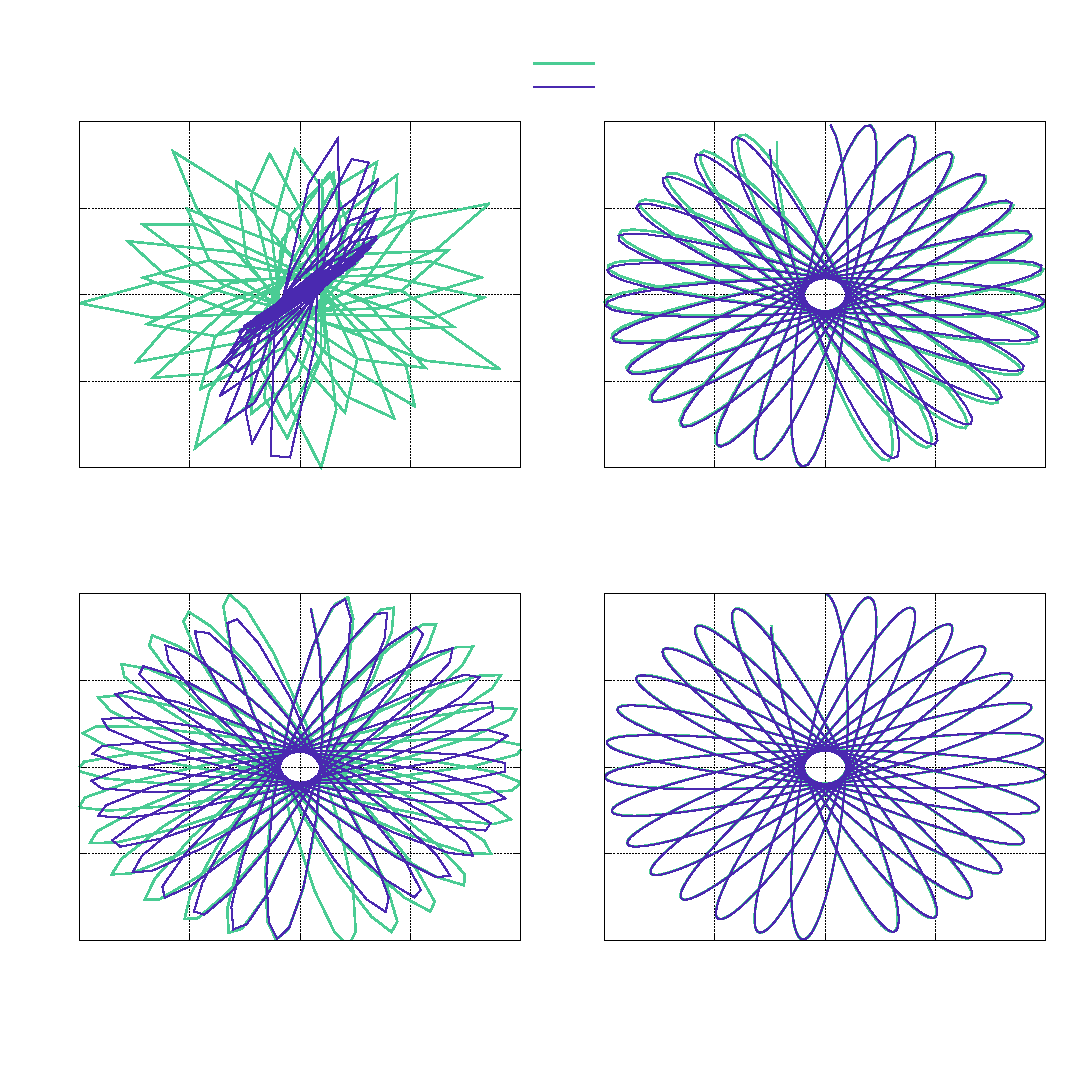
\includegraphics[width={504.00bp},height={504.00bp}]{plot}}%
    \gplfronttext
  \end{picture}%
\endgroup
